\chapter{Readout electronics and data acquisition}
\label{Chapter:ReadoutDAQ}


This~\cite{cepc_website} is an example with plots, please edit ... 
%
\begin{figure}[h!]
\centering
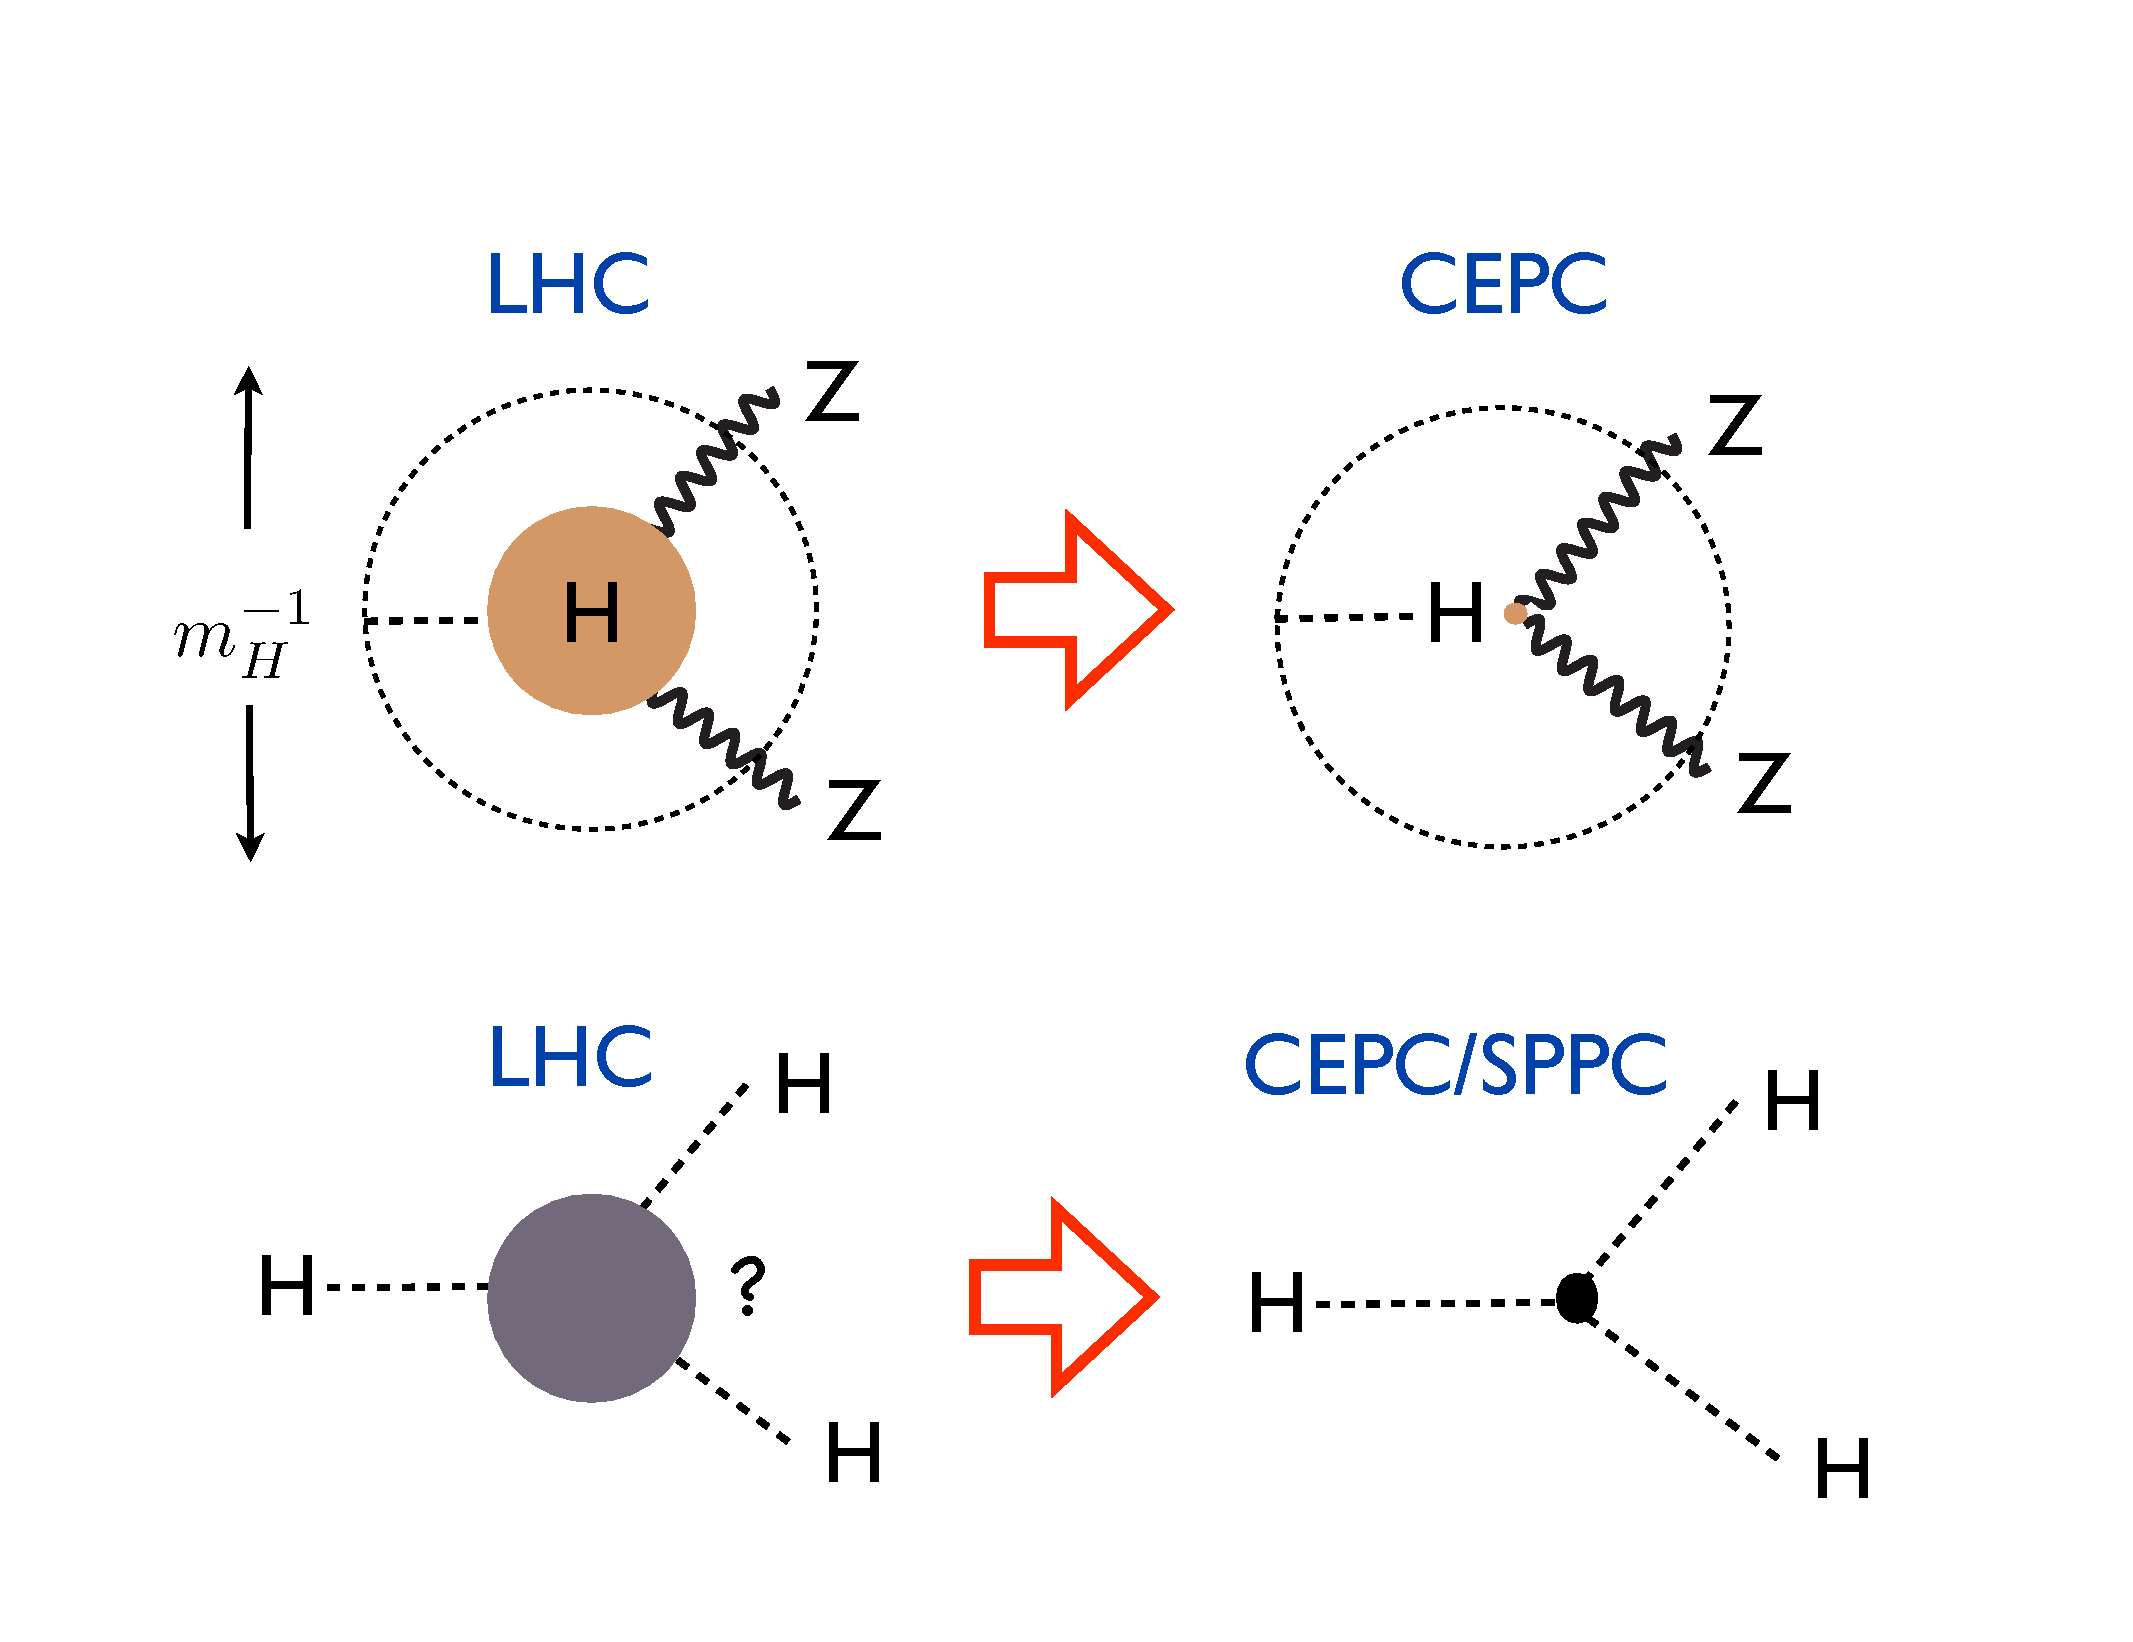
\includegraphics[scale=0.36]{Figures/ReadoutDAQ/main_theme}
\caption{A sketch of two of the central goals of the CEPC and SPPC. The CEPC will probe whether the Higgs is truly ``elementary", with a resolution up to a hundred times more powerful than the LHC. The SPPC will see, for the first time, a fundamentally new dynamical process --- the self-interaction of an elementary particle --- uniquely associated with the Higgs.}
\label{fig:main_theme}
\end{figure}
%
\section{New Colliders for a New Frontier}


\begin{figure}[h!]
\centering
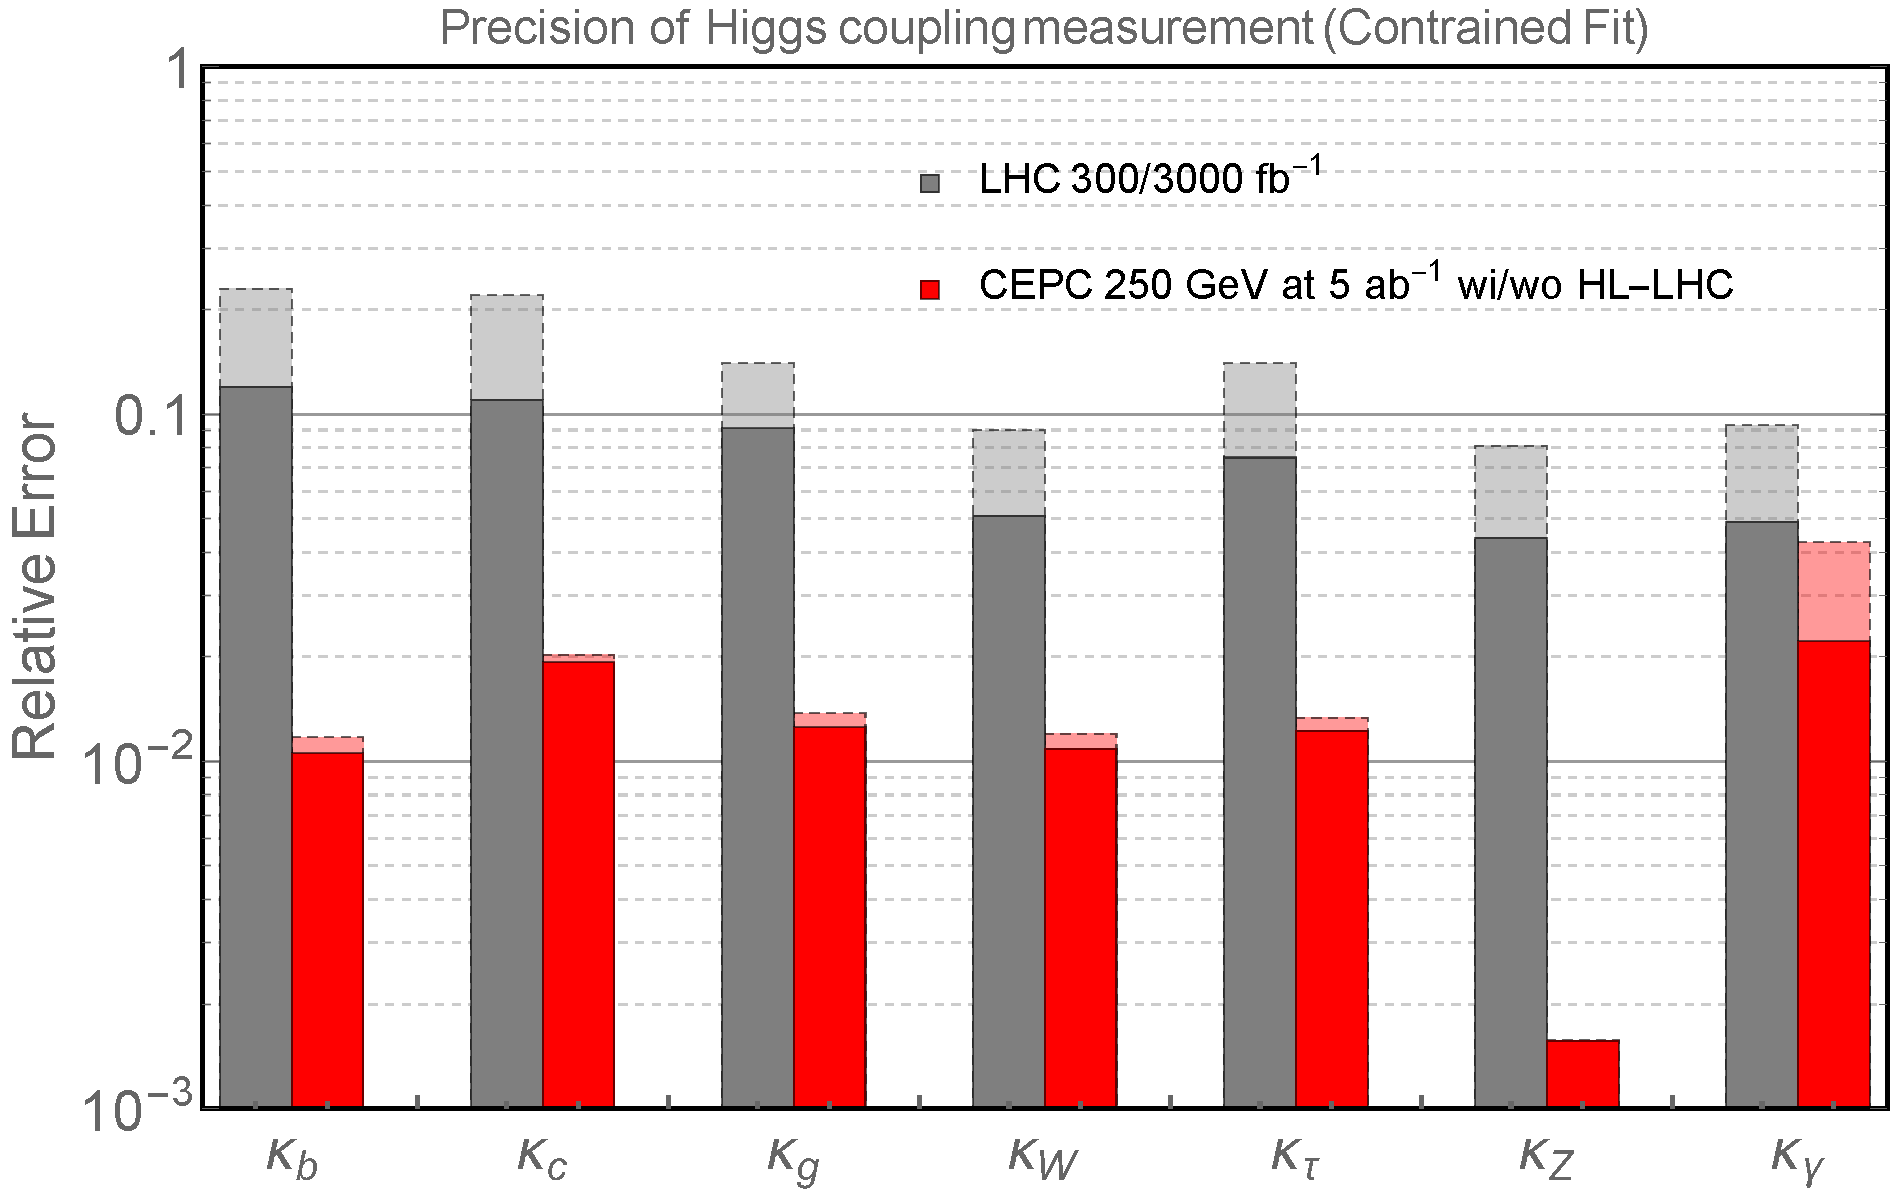
\includegraphics[scale=0.32] {Figures/ReadoutDAQ/7p_L_HL_CC.pdf}
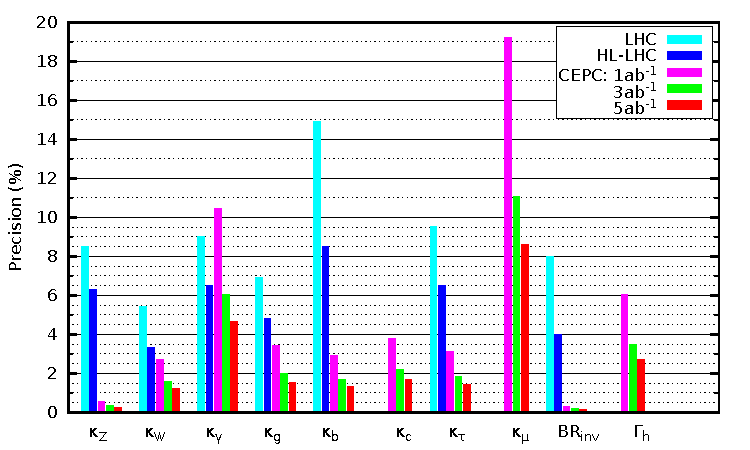
\includegraphics[scale=0.80] {Figures/ReadoutDAQ/fig_HCfit10.pdf}
\caption{Top: The 7 parameter fit, and comparison with the HL-LHC, discussed in detail in Chapter~\ref{Chapter:Higgs}. The projections for CEPC at 250 GeV with 5~ab$^{-1}$ integrated luminosity are shown. The CEPC results without combination with HL-LHC input are  shown with dashed edges. The LHC projections for an integrated luminosity of 300 fb$^{-1}$ are shown in dashed edges. Bottom: Comparison between the LHC and several benchmark luminosities of the CEPC. }
\label{fig:7param}
\end{figure}


\bibliographystyle{Style/atlasnote} %% plain.bst
\bibliography{Chapters/ReadoutDAQ} %% bsample.bib

